\part{Numerical Integrators}
\label{partNumericalMethods}

This analysis tool that models alveoli using dodecahedra requires numerical methods for performing integrations.  These numerical methods are discussed below.

\section{ODE Solvers}

The various constitutive equations that describe our alveolar model present themselves as ordinary differential equations that need to be integrated.  To this end, we employ the PECE (Predict, Evaluate, Correct, re-Evaluate) algorithms of Freed \cite{Freed17a} which are suitable for solving stiff systems of first- and second-order, ordinary, differential equations.  These methods are based upon Gear's well-known second-order backward difference formula (BDF2).

Time $t$ is considered to be the independent variable, discretized over an interval in time $[t_0,t_n]$ for which $N$ solutions are to be extracted at nodes $n=1, 2, \ldots, N$ spaced at uniform intervals in time with a common step size of $h = (t_n-t_0)/N$ separating them.  This is the \textit{global step size\/} at which solutions are to be gathered.  A dynamically controlled \textit{local step size}, whose size is adjusted to manage truncation error, is implemented into the code according to a scheme put forward in Ref.~\cite{Soderlind02}.  Solver interfaces are listed in \ref{appSolvers}.

\subsection{PECE Solver for First-Order ODEs}

Let $\mathbf{x}$ be a vector of dependent variables obeying a differential equation of evolution $\mathrm{d} \mathbf{x}(t) / \mathrm{d} t = \dot{\mathbf{x}} = \mathbf{f} (t, \mathbf{x})$ subject to an initial condition $\mathbf{x}_0 = \mathbf{x}(t_0)$.  One may think of $\mathbf{x}$ as being displacements whose rates $\dot{\mathbf{x}} = \mathbf{v}$ are velocities.  We find it useful to express $\dot{\mathbf{x}}$ as $\mathbf{v}$.

The method put forward here incrementally solves such an ODE, returning solutions associated with the next moment in time $t_{n+1}$, i.e., it acquires $\mathbf{x}_{n+1}$, given knowledge of the  previous $\mathbf{x}_{n-1}$ and current $\mathbf{x}_n$ solutions plus their rates $\mathbf{v}_{n-1}$ and $\mathbf{v}_n$ with the corrector also depending upon $\mathbf{v}_{n+1}$, i.e., the corrector is an implicit method.

\subsubsection{Start-Up Algorithm}

Multi-step methods are not self starting; consequently, Heun's method (a forward-Euler predictor with a trapezoidal corrector) is used here to start our integrator; specifically,
\begin{subequations}
    \label{startUp1stOrderODEs}
    \begin{align}
    \mbox{} & \text{Predict} & 
    \mathbf{x}_1^p & = \mathbf{x}_0 + h \mathbf{v}_0 + \mathcal{O} (h^2)
    \label{startUp1stOrderPredictor} \\
    \mbox{} & \text{Evaluate} & 
    \mathbf{v}^p_1 & = \mathbf{f} (t_1 , \mathbf{x}_1^p) 
    \label{startUp1stEvaluate} \\
    \mbox{} & \text{Correct} &
    \mathbf{x}_1 & = \mathbf{x}_0 + \tfrac{1}{2} h 
    \bigl( \mathbf{v}_1^p + \mathbf{v}_0 \bigr) + \mathcal{O} (h^3)
    \label{startUp1stOrderCorrector} \\
    \mbox{} & \text{Re-Evaluate} & 
    \mathbf{v}_1 & = \mathbf{f} (t_1 , \mathbf{x}_1) 
    \label{startUp1stReEvaluate}
    \end{align}
\end{subequations}
wherein $\mathbf{v}_0 = \mathbf{f}(t_0, \mathbf{x}_0)$ and $t_1 = t_0 + h$.  The correct\slash re-evaluate steps can be iterated over until a convergence criterion is satisfied, if need be.

\subsubsection{Two-Step ODE Solver}

The two-step method of Freed \cite{Freed17a} for solving $1^{\text{st}}$ order ODEs is
\begin{subequations}
    \label{1stOrderODEs}
    \begin{align}
    \mbox{} & \text{Predict} & 
    \mathbf{x}_{n+1}^p & = \tfrac{1}{3} 
    \bigl( 4 \mathbf{x}_n - \mathbf{x}_{n-1} \bigr) + 
    \tfrac{2}{3} h \bigl( 2 \mathbf{v}_n - \mathbf{v}_{n-1} 
    \bigr) + \mathcal{O} (h^3)
    \label{1stOrderPredictor} \\
    \mbox{} & \text{Evaluate} & 
    \mathbf{v}^p_{n+1} & = \mathbf{f} (t_{n+1} , \mathbf{x}_{n+1}^p) 
    \label{1stOrderEvaluate} \\
    \mbox{} & \text{Correct} &
    \mathbf{x}_{n+1} & = \tfrac{1}{3} 
    \bigl( 4 \mathbf{x}_n - \mathbf{x}_{n-1} \bigr) + 
    \tfrac{2}{3} h \mathbf{v}^{p}_{n+1} + \mathcal{O} (h^3)
    \label{1stOrderCorrector} \\
    \mbox{} & \text{Re-Evaluate} & 
    \mathbf{v}_{n+1} & = \mathbf{f} (t_{n+1} , \mathbf{x}_{n+1}) 
    \label{1stOrderReEvaluate}
    \end{align}
\end{subequations} 
where $t_{n+1} = t_n + h$.  This corrector is the well-known BDF2 formula of Gear to which Freed provided a predictor.  The correct\slash re-evaluate steps can be iterated over until a convergence criterion is satisfied, if need be.  Implementation of this integrator is found in \ref{app1stOrderODEs}.  

For both the predictor and corrector, solution $\mathbf{x}$ has a weight of 1, while its rate $\mathbf{v}$ has a weight of $\tfrac{2}{3} h$; hence, this predictor\slash corrector pair is consistent.

\subsection{PECE Solver for Second-Order ODEs}

Let $\mathbf{x}$ be a vector of dependent variables obeying a differential equation of evolution $\mathrm{d}^2 \mathbf{x}(t) / \mathrm{d} t^2 = \ddot{\mathbf{x}} = \mathbf{f} (t, \mathbf{x}, \dot{\mathbf{x}})$ subject to initial conditions $\mathbf{x}_0 = \mathbf{x}(t_0)$ and $\dot{\mathbf{x}}_0 = \dot{\mathbf{x}}(t_0)$.  One may think of $\mathbf{x}$ as being displacements and their rates $\mathbf{v} = \dot{\mathbf{x}}$ as being velocities with $\mathbf{a} = \dot{\mathbf{v}} = \ddot{\mathbf{x}}$ representing accelerations.  We find it useful to express $\dot{\mathbf{x}}$ as $\mathbf{v}$ and $\ddot{\mathbf{x}}$ as $\mathbf{a}$.

The method put forward here incrementally solves such an ODE, returning solutions associated with the next moment in time $t_{n+1}$, i.e., it acquires $\mathbf{x}_{n+1}$ \& $\mathbf{v}_{n+1}$ given knowledge of the previous $\mathbf{x}_{n-1}$ \& $\mathbf{v}_{n-1}$ and current $\mathbf{x}_n$ \& $\mathbf{v}_n$ solutions plus their accelerations $\mathbf{a}_{n-1}$ and $\mathbf{a}_n$ with the corrector also depending upon $\mathbf{a}_{n+1}$, i.e., the corrector is an implicit method.

\subsubsection{Start-Up Algorithm}

Multi-step methods are not self starting, so a one-step method is needed to take the first step of integration, specifically
\begin{subequations}
    \label{pairedStartUp}
    \begin{align}
    \mbox{} & \text{Predict} & 
    \mathbf{x}_1^p & = \mathbf{x}_0 + h \mathbf{v}_0 +
    \tfrac{1}{2} h^2 \mathbf{a}_0 + \mathcal{O} (h^3) 
    \label{startupDisplacementPredictor} \\
    \mbox{} & &
    \mathbf{v}^p_1 & = \mathbf{v}_0 + h \mathbf{a}_0 + 
    \mathcal{O} (h^2) 
    \label{startUpVelocityPredictor} \\
    \mbox{} & \text{Evaluate} &
    \mathbf{a}^p_1 & = \mathbf{a} (t_1, \mathbf{x}^p_1, \mathbf{v}^p_1)
    \label{startUpEvaluate} \\
    \mbox{} & \text{Correct} &
    \mathbf{x}_1 & = \mathbf{x}_0 + \tfrac{1}{2} h 
    \bigl( \mathbf{v}^p_1 + \mathbf{v}_0 \bigr) -
    \tfrac{1}{12} h^2 \bigl( \mathbf{a}^p_1 - 
    \mathbf{a}_0 \bigr) + \mathcal{O} (h^4) 
    \label{startupDisplacementCorrector} \\
    \mbox{} & &
    \mathbf{v}_1 & = \mathbf{v}_0 + \tfrac{1}{2} h 
    \bigl( \mathbf{a}_1^p + \mathbf{a}_0 \bigr) + 
    \mathcal{O} (h^3)
    \label{startUpVelocityCorrector} \\
    \mbox{} & \text{Re-Evaluate} &
    \mathbf{a}_1 & = \mathbf{a} (t_1, \mathbf{x}_1, \mathbf{v}_1) 
    \label{startUpReEvaluate}
    \end{align}
\end{subequations}
wherein $\mathbf{a}_0 = \mathbf{f}(t_0, \mathbf{x}_0, \mathbf{v}_0)$ and $t_1 = t_0 + h$.  The correct\slash re-evaluate steps can be iterated over until a convergence criterion is satisfied, if need be.

\subsubsection{Two-Step ODE Solver}

The two-step method of Freed \cite{Freed17a} for solving $2^{\text{nd}}$ order ODEs is
\begin{subequations}
    \label{pairedMethods}
    \begin{align}
    \mbox{} & \text{Predict} &
    \mathbf{x}_{n+1}^p & = \tfrac{1}{3} \bigl(
    4 \mathbf{x}_n - \mathbf{x}_{n-1} \bigr) + 
    \tfrac{1}{6} h \bigl( 3 \mathbf{v}_n + 
    \mathbf{v}_{n-1} \bigr) \notag \\ 
    \mbox{} & & & \hspace{3.175cm} + 
    \tfrac{1}{36} h^2 \bigl( 31 \mathbf{a}_n - 
    \mathbf{a}_{n-1} \bigr) + \mathcal{O} (h^4) 
    \label{displacementPredictor} \\
    \mbox{} & &
    \mathbf{v}_{n+1}^p & = \tfrac{1}{3} 
    \bigl( 4 \mathbf{v}_n - \mathbf{v}_{n-1} \bigr) + 
    \tfrac{2}{3} h \bigl( 2\mathbf{a}_n - \mathbf{a}_{n-1} 
    \bigr) + \mathcal{O} (h^3)
    \label{velocityPredictor} \\
    \mbox{} & \text{Evaluate} &
    \mathbf{a}^p_{n+1} & = \mathbf{a} (t_{n+1}, \mathbf{x}^p_{n+1}, \mathbf{v}^p_{n+1}) 
    \label{2ndEvaluate} \\
    \mbox{} & \text{Correct} & 
    \mathbf{x}_{n+1} & = \tfrac{1}{3} \bigl(
    4  \mathbf{x}_n - \mathbf{x}_{n-1} \bigr) +
    \tfrac{1}{24} h \bigl( \mathbf{v}^p_{n+1} +
    14 \mathbf{v}_n + \mathbf{v}_{n-1} \bigr) 
    \notag \\
    \mbox{} & & & \hspace{3.175cm} +
    \tfrac{1}{72} h^2 \bigl( 10 \mathbf{a}^p_{n+1} + 
    51 \mathbf{a}_n - \mathbf{a}_{n-1} \bigr) + 
    \mathcal{O} (h^4)
    \label{displacementCorrector} \\ 
    \mbox{} & &
    \mathbf{v}_{n+1} & = \tfrac{1}{3} 
    \bigl( 4 \mathbf{v}_n - \mathbf{v}_{n-1} \bigr) + 
    \tfrac{2}{3} h \mathbf{a}^p_{n+1} + \mathcal{O} (h^3)
    \label{velocityCorrector} \\
    \mbox{} & \text{Re-Evaluate} & 
    \mathbf{a}_{n+1} & = \mathbf{a} (t_{n+1}, \mathbf{x}_{n+1}, \mathbf{v}_{n+1})
    \label{2ndReEvaluate}
    \end{align}
\end{subequations}
where $t_{n+1} = t_n + h$.  An implementation of this integrator is described in \ref{app2ndOrderODEs}.  

The above PECE solver for velocity $\mathbf{v}$ is the same method presented in Eq.~(\ref{1stOrderODEs}), so this predictor\slash corrector pair is consistent.  Likewise, in both the predictor and corrector for displacement $\mathbf{x}$, contributions from the solution $\mathbf{x}$ have a weight of 1, contributions from the velocities $\mathbf{v}$ have a weight of $\tfrac{2}{3} h$, and contributions from the accelerations $\mathbf{a}$ have a weight of $\tfrac{5}{6} h^2$; hence, this predictor\slash corrector pair is consistent, too.

\section{Quadrature Rules for a Regular Pentagon}
\label{secGauss}

Three, Gauss, quadrature rules for a regular pentagon described in its natural coordinate system, i.e., oriented according to Fig.~\ref{figRegPentagon}, are presented in Table~\ref{tabQuadrature}.  These quadratures exactly integrate polynomials of order 1, 3 and 5, respectively.  They were supplied to the authors by Prof.\ N.\ Sukumar from the University of California at Davis, which he derived for us at our request using a methodology that he published in \cite{Mousavietal10}.  In that document, the authors derived formul\ae\ for determining the nodes and weights for a class of generalized, Gaussian, quadrature rules, which they then applied to pentagons, hexagons, heptagons and octagons, of which they only published their nodes and weights of quadrature for the hexagon, as it tiles two space.  The node for the $1^{\mathrm{st}}$ order method is located at the centroid of the pentagon.  Nodes for the $3^{\mathrm{rd}}$ and $5^{\mathrm{th}}$ order methods of Table~\ref{tabQuadrature} are displayed in Fig.~\ref{figQuadrature}.

\begin{table}
    \centering
    \begin{tabular}{|c|rrr|}
        \hline
        node & \centering $\xi$ coordinate \phantom{123}  & 
        $\eta$ coordinate \phantom{123} & weight \phantom{12345} \\ \hline
        & \multicolumn{3}{|c|}{Exact for Polynomials of Degree $1^{\phantom{|^|}}$} \\ \hline
        1 & 0.0000000000000000 & 0.0000000000000000 &
        2.3776412907378837\vphantom{$|^{|^|}$} \\ 
        \hline
        & \multicolumn{3}{|c|}{Exact for Polynomials of Degree $3^{\phantom{|^|}}$} \\ \hline
        1 & -0.0349156305831802 &  0.6469731019095136 &
        0.5449124407446143\vphantom{$|^{|^|}$} \\
        2 & -0.5951653065516678 & -0.0321196846022659 & 0.6439082046243272 \\
        3 &  0.0349156305831798 & -0.6469731019095134 & 0.5449124407446146 \\
        4 &  0.5951653065516677 &  0.0321196846022661 & 0.6439082046243275 \\ 
        \hline
        & \multicolumn{3}{|c|}{Exact for Polynomials of Degree $5^{\phantom{|^|}}$} \\ \hline
        1 & -0.0000000000000000 & -0.0000000000000002 &
        0.6257871064166934\vphantom{$|^{|^|}$} \\
        2 & -0.1351253857178451 &  0.7099621260052327 & 0.3016384608809768 \\
        3 & -0.6970858746672087 &  0.1907259121533272 & 0.3169910433902452 \\ 
        4 & -0.4651171392611024 & -0.5531465782166917 & 0.3155445150066620 \\
        5 &  0.2842948078559476 & -0.6644407817506509 & 0.2958801959111726 \\
        6 &  0.7117958231685716 & -0.1251071394727008 & 0.2575426306970870 \\
        7 &  0.5337947578638855 &  0.4872045224587945 & 0.2642573384350463 \\
        \hline
    \end{tabular}
    \caption{Generalized, Gaussian, quadrature, weights and nodes (a.k.a., cubature rules) for integrating over a regular pentagon in its natural coordinate system.  These weights sum to the area of a pentagon inscribing an unit circle.}
    \label{tabQuadrature}
\end{table}

The Gaussian quadrature rules of Mousavi, Xiao \& Sukumar \cite{Mousavietal10} presented in Table~\ref{tabQuadrature} are compatible with the shape functions of Wachspress \cite{Wachspress75,Wachspress16} and Dasgupta \cite{Dasgupta03} presented in \S\ref{secShapeFns}.

\begin{figure}
    \centering
    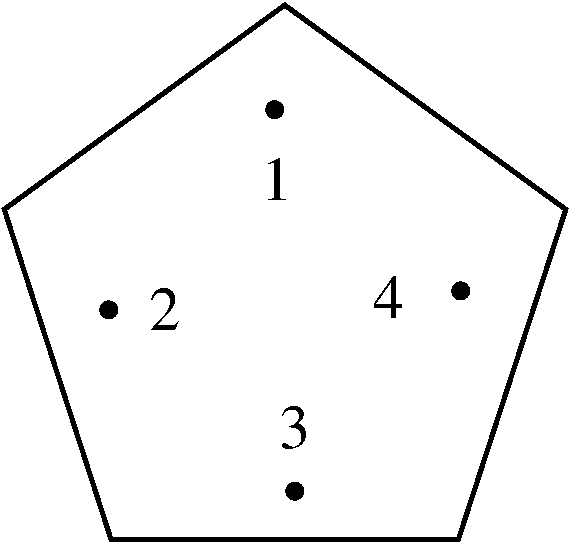
\includegraphics[width=6cm]{figures/pentagon_degree3.pdf}
    \hspace{1cm}
    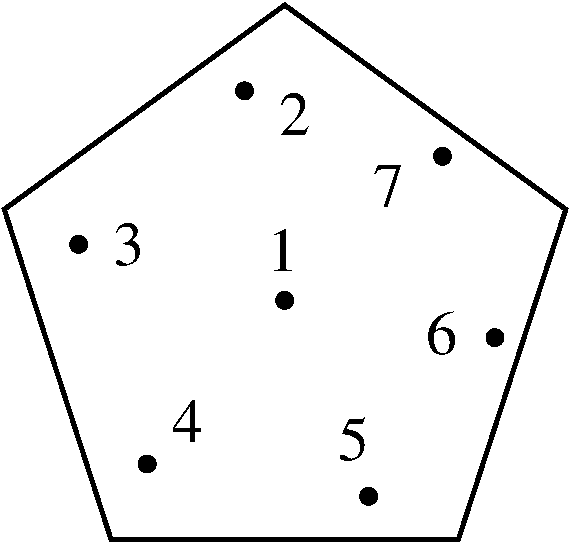
\includegraphics[width=6cm]{figures/pentagon_degree5.pdf}
    \caption{Locations of generalized, Gaussian, quadrature nodes for the $3^{\mathrm{rd}}$ (left) and $5^{\mathrm{th}}$ (right) degree integration methods presented in Table~\ref{tabQuadrature}.  Vertex 1 is located at the top of the pentagon, cf.\ Fig.~\ref{figRegPentagon}, while the coordinate origin is located at its centroid (node 1 in the right figure).}
    \label{figQuadrature}
\end{figure}
